\section{Objective}
\subsection{Objective and Premise of the Design Project }
The design project is based on the case as presented by DMA entitled “Digital One-Day Courses for Doctors” <Reference to the case description as an appendix?>. The direct goal of the case description is the development of a “digital learning platform”. The motivation is to provide to the more than 27000 members (per January 1. 2014) more courses on demand and give them an overview of available online courses both nationally and internationally.

The DMA had a focus group develop requirements for the platform and easy access triumphed over variety, looks and features as the most important consideration. Additionally, the case asks us to consider the following:

\begin{enumerate}[A.]
\item Will there be in a foreseeable future sufficient demand for digital learning services and/or platform from DMA members?
\item What do the end users require from a digital learning platform?
\item How can a digital learning platform be implemented within the existing organisation of DMA?
\item What is the ‘minimal viable product’ i.e. the most simple inexpensive product that allows DMA to enter this market?
\end{enumerate}

And in the pursuit of these to explore:

\begin{itemize}
\item What are the reasons for the current lack of incitement for the digital offers?
\item How can digital learning  be embedded in the daily work of doctors, who typically demand a decent work-life balance, and who typically prefer education to be something that happens in a formal setting such as a course or conference?
\item Is it more suitable continuing the current ad-hoc strategy, or does the increased uptake of digital learning offer a more holistic, top-down strategy and thus also a platform?
\item What devices will best support the learning situation: Computers, tablets or smart phones, or should the solution be compatible with all types of devices?
\end{itemize}

DMAs expectations to the solution were:

\begin{itemize}
\item A specification of a strategy that will provide the members of the DMA with more digital learning possibilities. This includes considerations about the cost structure, resource requirements etc.
\item A specification of the user requirements and design of a digital learning service offers that sufficiently fit with the existing organisation in DMA.
\item A design proposal for the learning service, including considerations regarding distribution of this.
\item A specification of the overall technical requirements for such a solution, including recommendations for the software platform, and considerations regarding integration with the existing web page www.laeger.dk.
\item Considerations regarding channels for distribution of the service (e.g. via the existing homepage or via app stores).
\end{itemize}

We had some ideas to what might fulfil the noted requirements as we started the project. The main idea we discussed was an e-learning platform where courses were “chopped up” into 5 minute bits that would be easy for the doctors to fit in and follow in their busy schedules. <Don’t know where else to fit this in?>\footnote{TODO: FIX THIS}

In the initial phase of the MUST method, our approach was to establish a thorough understanding of the organisational setup of DMA and identify the main stakeholders. This allowed us to understand the scope of the project and eliminate all potential misunderstandings between the project group and the steering committee. In the first meeting with the steering committee , which consisted of Lene Rybner as the sole member, we got to know the project better and what the wishes and expectations of DMA were.

Based on our understanding and expectations at the time, we made a baseline plan for the project <Figure reference, insert figure below>\footnote{TODO: FIX THIS}. The deadlines and outcome of each phase of the project was dictated by the course structure, so this was unchanged, but we later made an updated baseline plan <Figure reference>\footnote{TODO: FIX THIS} that describes the actual activities in each phase.


\section{In-line Analysis Phase}
\subsection{Approach}
Our approach in the in-line analysis phase was to, firstly, figure out the major work domains to get a sense of where the IT system was used and where innovation could actually be required, and secondly, dig a little deeper into DMA’s organization by discovering some of their business strategies behind course creation, how are they created, who provides them and what are the main platforms of the courses.

\subsection{Environment}

The Danish Medical Association (DMA), Lægeforeningen in Danish, is an association that aims to represent all Danish doctors and their associated organisations such as unions, tying them all together and providing benefits for all its members. There are three major medical organisations under the DMA. The structure is illustrated in figure \ref{fig:dmaorganisation}.

The first is “Yngre Læger” (YL), an association for younger doctors with close ties to doctors advancing their studies in the “klinisk basisuddannelse” (KBU), those taking their introduction to their speciality and those who are actively specialising.

The second is “Forening af Speciallæger” (FAS) which is a union for consulting doctors that have studied a speciality.

Lastly is “Praktiserende Lægers Organisation” (PLO) which is an organisation for the practicing family doctors, who usually run their own local clinic for the nearby population.

Danish doctors are generally associated with one of these three organisations and are thus members of the DMA, having access to the DMA provided courses and other benefits.

\begin{figure*}[h!]
 \begin{center}
  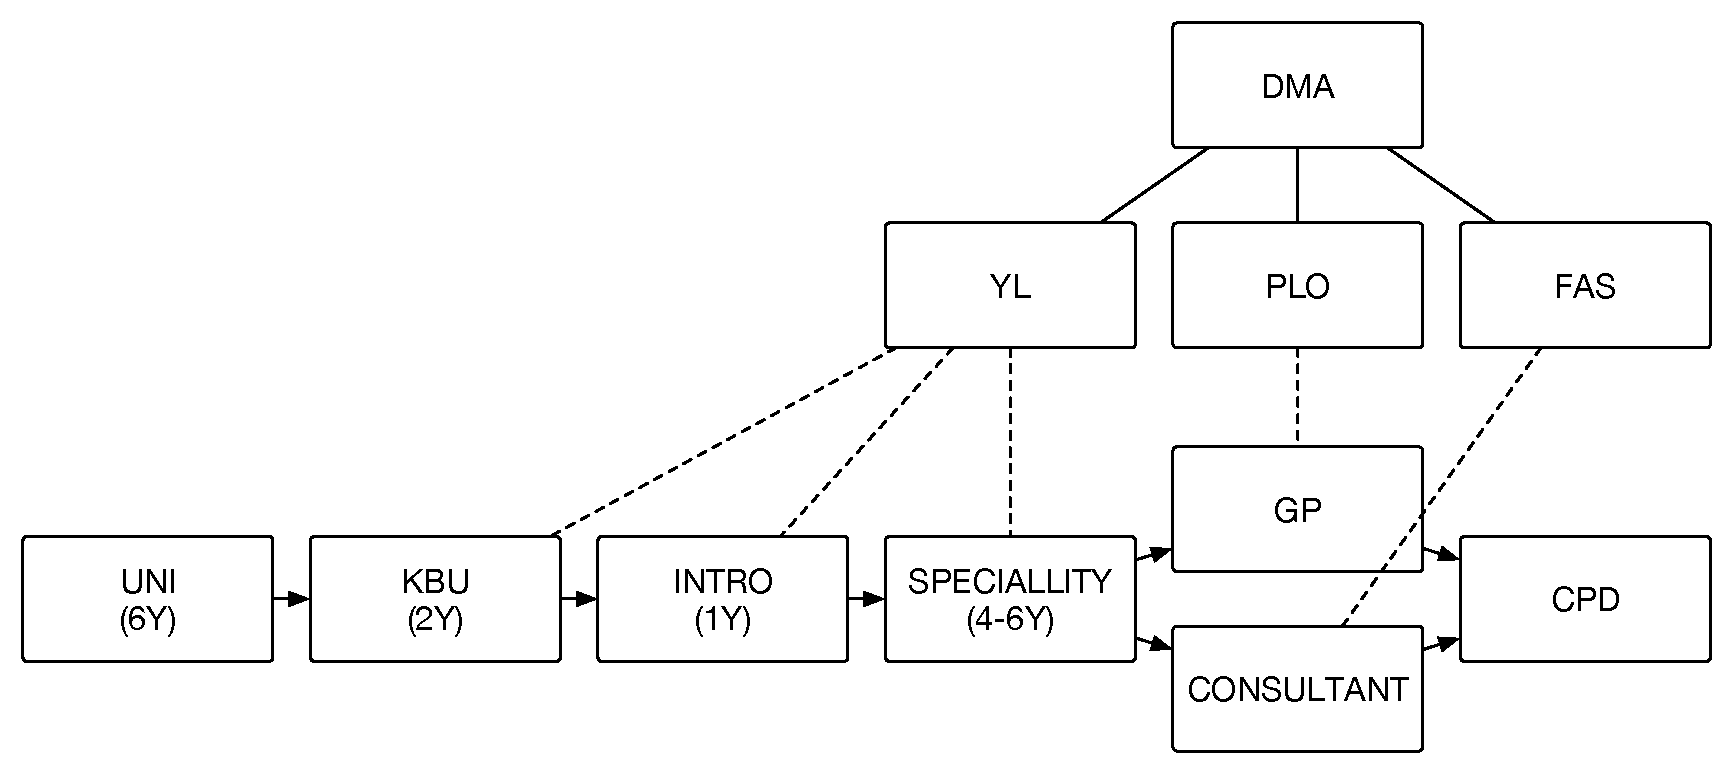
\includegraphics[width=1\textwidth]{figures/dma-structure.pdf}
  \caption{The organisation of DMA.\label{fig:dmaorganisation}}
 \end{center}
\end{figure*}

\subsubsection{Potential and Needs}
DMA members need to take courses in order to stay up to date with the latest information about medicine practices. So far the existing e-learning platforms that provide the necessary courses are not widely used by the doctors, in some cases this is because they consider it to be time consuming. Some doctors also consider the contents of the e-learning courses to be too easy and superficial <Reference?>. What is needed is a new way to deliver information to the doctors, such that we can engage them in a way that eliminates the concerns of the current e-learning solutions.


\subsubsection{Requirements and Conditions}
DMA members are looking for a new e-learning platform with a different approach compared to the existing offers provided by DMA, such as BMJ Learning, since the DMA members do not currently utilise the offers as much as expected. DMA would like to have the content focused on including the entire spectrum (known as the 7 roles of physicians) of knowledge areas, which a modern doctor should be educated in, for example there should be topics dealing with communication, administration and so on. Currently surveys performed by DMA show that some doctors prefer to strictly focus their education on medical expertise and entirely neglecting being educated in the remaining 6 roles.

\subsubsection{Business Strategy}
\begin{description}
\item[Goals:] We aim to find an approach for busy doctors to learn course material that will work for them. The approach should be realistic and feasible within the constraints of the target association DMA, and should actually engage the doctors and fit their needs such that the doctors will use it in practice.
\item[Business Processes:] We did not consider business processes very relevant in this phase of the project. DMA has a dominant market position with 98\% of Danish doctors being members and a fixed membership fee subscription model, which was something we learned later.

We do not consider business processes relevant at this time, as it is outside the scope of our study.
\item[Challenges and Problems:] There are various challenges associated with solving the problem of doctors not actively continuing their education despite attempts to facilitate their learning. Firstly, we had to establish what was actually causing the problem. The cause seems to be that the doctors do not have time in their busy schedules to take hours or entire days off to study and take courses, but is this actually the main cause? Is there more to it? Are other factors in the way of doctors keeping up with their fields?

If the stated problem is confirmed to be what it seems to be, then we still have the problem of figuring out an alternative method of providing the course materials in a manner that is accessible to the doctors. And even with accessible learning, the approach still needs to motivate the doctors to actually use the solution. So we need to understand exactly what the doctors are looking for in a way of consuming courses and what exactly will suit their needs.
\end{description}

\subsection{Work Domains}
We have identified two primary work domains: Course creation and Doctors practice.

\textbf{Course Creation}
\begin{description}
\item[Definition:] The course creation work domain is the source that DMA uses to provide material for their members to educate themselves. It is not limited to the creators that DMA is directly linked with, but also external third party creators.

\item[Characterization:] DMA has multiple sources of courses and material of differing types and they are delivered in different ways, from BMJ’s e-learning platform, DMA’s own courses and courses created elsewhere and communicated to members through and by DMA.
The sources have different delivery methods, course content, evaluation methods and purpose.

DMA primarily uses their website and other IT based channels to inform their members of the existence of these courses, and to some extent also give access to them, for example by providing discounted membership fees to BMJ’s e-learning platform.
\item[Discussion/Conclusion:] The constraints and methods in course creation are key to determining what is possible to actually do in terms of innovative ideas.

\end{description}

\textbf{Doctors Practice}
\begin{description}
\item[Definition:] The actual work practice and daily schedule of DMA’s members, the doctors, and how much time and resources they have available for learning new things. This means both considering the day to day work schedule and any time dedicated to learning.

\item[Characterization:] Although DMA serves a very diverse member group, there is some common ground and work practices among a large part of their members. The doctors have a busy working day that is not very flexible, making it difficult for them to make time for the current format of provided courses.

Additionally some members lack incentive to prioritise learning over working, as some doctors are paid to learn, others are not.

\item[Discussion/Conclusion:] Whatever the quality of the courses provided by DMA may be, the doctors have to be able to find the time to take them. The courses also need to cater for the actual interests of the doctors and be relevant in their daily work.


\end{description}


\section{In-depth Analysis Phase}
\subsection{Approach}
Based on the results of the in-line analysis phase we interviewed a doctor who was also a course creator, sent out a questionnaire to a range of doctors and interviewed our key spokesperson at DMA, Lene Rybner. We intended to do work practice observations of doctors, but this proved too difficult to set up and we abandoned this in favor of the questionnaires and further interviews with Lene.

\subsection{Work Practices}
From an interview with a person who is both a doctor and a course creator of CPD material the project group was able to identify work practices at both ends of the table and help view the project from two different points of views.

We started asking her questions with regards to her role as a course creator. She had helped creating and managing a course on genetics, which she ran as an introductory course to raise awareness of genetics being a fully fledged medical field. The online platform chosen for the course was itslearning where all course material, exams and discussions were kept. This course had previously failed to start twice due to lack of participants.
Once they started using the DMA’s monthly email newsletter instead of a system that required a login (itslearning) to post the information about the course, they gathered enough participants.

We then switched question topics and started asking her questions with regards to her role as a doctor. When we asked if she would have 5 or 10 minutes of spare time at some point in her schedule, if she could see herself taking a fragment of an e-learning course, her answer was that the material would have to be very accessible. She has signed up for BMJ before but the slightest resistance such as a complicated login to a different system kills the “will to learn” moment.

The email newsletter is therefore a critical channel in engaging doctors and it makes good sense based on their current work practices. The email does not require a complicated login and it is right there in front of them when the doctor uses his/her computer. Doctors are usually too busy with other things on their mind than logins to different systems, so the accessibility to the course material is a critical point as well.

Throughout our interviews with Lene, we discovered that she is the one responsible for making the available courses or material known to the doctors’ community. She has created various accounts on social networks (Facebook, LinkedIn), through which she promotes various courses that are available on DMA, BMJ, MOOCs and other e-learning platforms. In our last meeting we discussed about what would be the preferable time limit for an online course, we suggested a 7 minute time limit  and she replied that it is too much for the doctors to spend that amount of time.

In order to suggest various courses to the doctors she has to search through the courses herself in the above mentioned sites and post them on Facebook groups and various home pages that doctors visit. Lately she has started posting pictures concerning medical problems that are not “graphic” as she stated, but interesting enough to make the doctors look up the courses she suggests. However, she has no way of knowing if her methods work, because everything is hosted in websites that are not hosted by DMA (Facebook, LinkedIn), hence she cannot have any information about the traffic.

\subsection{Course Participants}
\label{indepth:questionnaire}
In addition to the interviews we also sent out a questionnaire. We would have liked to interview many more people, but due to limited resources this was not feasible, and so a questionnaire provided a good means of looking into the needs of a group of actual doctors in the DMA. The group of DMA doctors we had access to were those who had participated in the Genetics Course provided by the DMA, which we were also given access to in our case study. Of these, 6 participants consented to participating in our questionnaire. However, at the time of this writing only 2 have responded. We would have liked to get in contact with many, many more doctors of varying background but, as discussed earlier, we had to prioritise our limited resources and so our reach was limited. Thus our analysis is based on less participants than we would have liked. Another pitfall of this particular questionnaire study is that we are only focusing on doctors that have been enrolled in a DMA course, and thus there might be a segment of doctors whose perspective is not addressed here.

Our aggregated findings along with the raw answers from the questionnaire can be found in appendix \ref{questionnaire}\footnote{TODO: FIX ME}, but a couple of points of particular note was that they find courses for their continuous professional education through Lægeforeningen, and that they are working at least full time with very busy schedules, from which they have to clear out entire days in order to attend courses. This tells us that Lægeforeningen is, in actual current work practices, a good place for doctors to find educational courses. It also confirms the “assumed” busy schedule of doctors and therefore the need to find something that fits into their busy work day.

\subsection{Goals, Problems, Needs, and Ideas for Solutions}

The solution we propose is influenced by our newly focused scope: the doctor’s time. Already there are a lot of courses available for doctors to choose from whether it’s from DMA, BMJ or MOOCs. As mentioned before, the project group’s assumption is that the doctors are too busy to find out themselves which courses are relevant to their CPD. The problem is not that doctors don’t want to take the courses or use e-learning platforms, but more of that they are not properly introduced to available courses. We propose creating a well-defined framework for the DMA to work within to help them to sell the courses by using something we call a course hook.

In the in-depth analysis phase we discovered that the DMA’s newsletter was important. Based on our focused scope on the doctor’s time, one solution would be that the DMA itself would pick out a subset of available courses from the vast variety of course material and advertise them in the newsletter based on medicine specialities. By using our terms before, we can give an example:


\begin{center}
“How well do you know Genetics?” (\textbf{Headline})

[VIDEO] A 5 minute introduction to the upcoming course in Genetics (\textbf{The hook})
\end{center}

In this example, the DMA has handpicked a course on Genetics which they feel is a very appropriate course for genetics. There is a number of important things in this example. First, the advertisement is selling a genetics course and does so by challenging the doctor’s knowledge. Second, the doctor can see exactly what kind of introduction this is and how long it takes (the hook). The doctors are therefore able to make a decision based on their strict schedule whether or not they have spare time.

In \ref{section:visions_change}\footnote{TODO: FIX ME} we talk about this method in detail.

